% Created 2026-03-26 qui 14:53
% Intended LaTeX compiler: lualatex
\documentclass[12pt,a4paper]{article}
\usepackage{fgv-paper}
\usepackage{float}
\usepackage{graphicx}
\usepackage{caption}
\usepackage{xcolor}
\usepackage{tikz}
\usepackage{fancyhdr}
\usepackage{tcolorbox}
\usepackage{tabularray}
\usepackage{booktabs}
\usepackage{tabularx}
\usepackage{array}
\usepackage{longtable}
\usepackage{ltablex}
\keepXColumns
\setlength{\emergencystretch}{3em}
\sloppy
\definecolor{FGVHeaderBlueDark}{HTML}{003A70}
\definecolor{FGVHeaderBlueMid}{HTML}{005AA9}
\definecolor{FGVHeaderBlueLight}{HTML}{66A9E0}
\setlength{\headheight}{48pt}
\setlength{\headsep}{12pt}
\newcommand{\FGVHeaderLogoInclude}{
\includegraphics[height=0.95cm]{/home/gustavodetarso/Documentos/.share/mgs_org/fgv.png}}
\newcommand{\FGVHeaderGradientRule}{\begin{tikzpicture}[baseline=(current bounding box.center)]\shade[left color=FGVHeaderBlueDark,middle color=FGVHeaderBlueMid,right color=FGVHeaderBlueLight] (0,0) rectangle (\headwidth,1.2pt);\end{tikzpicture}}
\newcommand{\FGVHeaderBlock}{\begin{minipage}[b]{\headwidth}\raggedright \FGVHeaderLogoInclude\par\vspace{0.18em}\noindent\FGVHeaderGradientRule\end{minipage}}
\fancypagestyle{fgvreportstyle}{%
\fancyhf{}%
\fancyhead[L]{\makebox[\headwidth][l]{\FGVHeaderBlock}}%
\fancyhead[C]{}%
\fancyhead[R]{}%
\renewcommand{\headrulewidth}{0pt}%
\fancyfoot[C]{\thepage}%
}
\fancypagestyle{plain}{%
\fancyhf{}%
\fancyhead[L]{\makebox[\headwidth][l]{\FGVHeaderBlock}}%
\fancyhead[C]{}%
\fancyhead[R]{}%
\renewcommand{\headrulewidth}{0pt}%
\fancyfoot[C]{\thepage}%
}
\AtBeginDocument{\pagestyle{fgvreportstyle}\thispagestyle{fgvreportstyle}}
\author{Gustavo M. Mendes de Tarso}
\date{\today}
\title{}
\hypersetup{
 pdfauthor={Gustavo M. Mendes de Tarso},
 pdftitle={},
 pdfkeywords={},
 pdfsubject={},
 pdfcreator={Emacs 28.2 (Org mode 9.5.5)}, 
 pdflang={Pt_Br}}
\usepackage[style=backend=biber,style=apa,sortcites=true,sorting=nyt,giveninits=true,maxcitenames=2,maxbibnames=20,uniquelist=minyear]{biblatex}
\addbibresource{/home/gustavodetarso/Documentos/mppg/disciplinas/teorias_da_administração_publica/criador_de_atividade/pesquisas/atividade_uso_da_inteligencia_artificial_na_administracao_publica_federal_em_governanca_integridade_e_gestao_de_riscos_prisma/atividade_uso_da_inteligencia_artificial_na_administracao_publica_federal_em_governanca_integridade_e_gestao_de_riscos_prisma.bib}
\begin{document}

\begingroup
\linespread{1}\selectfont
\begin{tcolorbox}[title=Ficha Técnica,
  colback=gray!5,colframe=gray!40,boxrule=0.4pt,sharp corners]
\begin{tblr}{rowsep=1pt,stretch=1, rows={t}, colspec={Q[l,2.8cm] X[l]}}
\textbf{Curso}                   & Mestrado em Políticas Públicas e Governo \\
\textbf{Turma}                   & 2026.1 \\
\textbf{Pólo}                    & Brasília \\
\textbf{Disciplina}              & Teorias da Administração Pública \\
\textbf{Professor}               & Bernardo Buta \\
\textbf{Aluno(s)}                & Hugo Bustomante Tre \\
\textbf{Data}                    & 24 de março de 2026 \\
\textbf{Título do trabalho}      & Uso da inteligência artificial na administração pública federal em governança, integridade e gestão de riscos \\
\end{tblr}
\end{tcolorbox}
\endgroup

\clearpage

\section{Introdução}
\label{sec:org8b8e088}

Esta triagem tem por finalidade identificar, entre os resultados recuperados nas bases Semantic Scholar e Scopus, um estudo empírico que dialogue de modo mais aderente com o tema do uso da inteligência artificial na administração pública federal em governança, integridade e gestão de riscos. Considerando o objetivo da atividade acadêmica, priorizaram-se trabalhos publicados entre 2020 e 2026, em português ou inglês, com texto completo verificável, e que apresentassem aplicação concreta, avaliação empírica, estudo de caso, survey, análise quantitativa, métodos mistos ou exame de implementação institucional. Adicionalmente, buscou-se maior proximidade com organizações públicas, mecanismos de transparência, accountability, integridade, auditoria, fiscalização, prevenção de corrupção e apoio à decisão. Embora o recorte privilegie a administração pública federal brasileira, o conjunto recuperado mostrou predominância de estudos internacionais e, em muitos casos, de natureza conceitual ou de revisão. Assim, a seleção final considerou a melhor combinação entre aderência temática, natureza empírica, presença de aplicação em setor público e disponibilidade verificável de texto completo.

O artigo selecionado ao final do processo foi \textbf{“Automating public governance oversight: Evidence from the Federal District of Brazil”}. A escolha final se justifica porque O artigo "Automating public governance oversight: Evidence from the Federal District of Brazil" foi selecionado por apresentar a combinação mais forte entre aderência temática, natureza empírica e aplicabilidade ao recorte da atividade. Trata-se de um estudo empírico com abordagem de métodos mistos, baseado em análise documental, extração automatizada de dados e validação de conteúdo em 47 entidades públicas, examinando como automação e inteligência artificial podem fortalecer transparência, governança e monitoramento institucional. Seus achados dialogam diretamente com governança, accountability, supervisão automatizada e maturidade institucional, dimensões centrais para a integridade e a gestão de riscos no setor público. Embora o caso empírico esteja situado no Distrito Federal, ele se aproxima do contexto brasileiro de administração pública e oferece maior transferibilidade analítica para o debate sobre administração pública federal do que estudos internacionais excessivamente gerais ou exclusivamente normativos. Além disso, o registro informa full\_text\_verified=true e disponibiliza link de download verificável do texto completo em PDF (\url{https://ramp.ase.ro/vol45/45-05.pdf}), atendendo explicitamente à exigência metodológica de acesso verificável ao artigo completo.

Também é importante registrar uma distinção metodológica. Neste trabalho, o \textbf{PRISMA 2020} foi utilizado para organizar o \textbf{fluxo da busca e da seleção} nas bases consultadas \autocite{prisma2020statement}. O artigo selecionado foi analisado a partir de seus metadados e, obrigatoriamente, de um \textbf{texto completo com link verificável para download} \autocite{freire2025automating}.

\section{Estratégia de busca}
\label{sec:org4fc0624}

\subsection{Pergunta orientadora}
\label{sec:orgba9109e}

\begin{quote}
Como a inteligência artificial tem sido utilizada como instrumento de apoio à governança, à integridade e à gestão de riscos na administração pública, com ênfase em evidências empíricas aplicáveis ao contexto da administração pública federal?
\end{quote}

\subsection{Bases consultadas}
\label{sec:org302f09e}

\begin{itemize}
\item Semantic Scholar, Scopus
\end{itemize}

\subsection{Base e lógica de busca}
\label{sec:org67e5478}

A lógica de busca combinou três eixos: (i) tecnologia de interesse ("artificial intelligence" OR "inteligência artificial"); (ii) contexto organizacional ("federal public administration" OR "administração pública federal" OR "public sector" OR "setor público" OR government); e (iii) dimensões analíticas do recorte (governance OR governança OR integrity OR integridade OR "risk management" OR "gestão de riscos"), associados ainda a marcadores de desenho empírico ("empirical study" OR empirical OR empírico OR "case study" OR "estudo de caso" OR "implementation evaluation"). Na etapa de triagem, a decisão concentrou-se na aderência do resumo ao recorte substantivo e metodológico, distinguindo estudos empíricos de revisões, ensaios conceituais, análises normativas e textos fora do setor público ou fora do problema de governança, integridade e gestão de riscos.

\subsection{Queries por base}
\label{sec:org8a2f525}

\begin{itemize}
\item \textbf{Semantic Scholar}: \texttt{artificial intelligence federal public administration governance integrity risk}
\item \textbf{Scopus}: \texttt{TITLE-ABS-KEY(("artificial intelligence" OR "inteligência artificial") AND ("federal public administration" OR "administração pública federal" OR "public sector" OR "setor público" OR government) AND (governance OR governança OR integrity OR integridade OR "risk management" OR "gestão de riscos") AND ("empirical study" OR empírico OR empirical OR "case study" OR "estudo de caso" OR "implementation evaluation"))}
\end{itemize}

\subsection{Critérios de inclusão}
\label{sec:orga846610}

\begin{itemize}
\item Publicação entre 2020 e 2026.
\item Idioma em português ou inglês.
\item Texto completo verificável, com link de download acessível e full\_text\_verified=true.
\item Estudo relacionado ao uso de inteligência artificial na administração pública ou no setor público.
\item Foco substantivo em governança, integridade, transparência, accountability, auditoria, fiscalização, gestão de riscos, conformidade ou apoio à decisão pública.
\item Prioridade para estudos empíricos, tais como estudo de caso, survey, métodos mistos, análise quantitativa, análise documental empírica ou avaliação de implementação.
\item Preferência por estudos com maior proximidade à administração pública federal ou com potencial analítico de transferência para esse contexto.
\end{itemize}

\subsection{Critérios de exclusão}
\label{sec:orgf3dd611}

\begin{itemize}
\item Estudos sem relação com administração pública ou setor público.
\item Estudos centrados em educação, saúde clínica, mercado privado, finanças privadas, urbanismo geral, meio ambiente ou outros domínios sem conexão suficiente com governança pública, integridade ou gestão de riscos.
\item Revisões de literatura, ensaios teóricos, textos filosóficos, análises puramente normativas ou conceituais, quando houver alternativa empírica mais aderente.
\item Estudos focados exclusivamente em governos locais, municipalidades ou contextos muito específicos sem contribuição suficiente para o recorte pretendido.
\item Textos cujo foco principal não seja inteligência artificial aplicada à governança, integridade, fiscalização, controle, transparência ou gestão de riscos no setor público.
\item Registros com baixa aderência temática ao objetivo da atividade, ainda que tratem de IA de forma ampla.
\end{itemize}

\subsection{Observações de execução}
\label{sec:org4363205}

\begin{itemize}
\item Excluído antes da triagem por falta de texto completo verificável: Generative artificial intelligence in public administration: an integrated framework for regulatory compliance, ethical governance, and digital transformation.
\item Excluído antes da triagem por falta de texto completo verificável: Ethical Governance of Artificial Intelligence in Cardiovascular Disease Management: A Health Policy Perspective.
\item Excluído antes da triagem por falta de texto completo verificável: Advanced artificial intelligence at a corporate responsibility crossroads: employees as risk management advocates.
\item Excluído antes da triagem por falta de texto completo verificável: Artificial Intelligence in Public Administration: A Systematic Literature Review on Opportunities and Ethical Challenges.
\item Excluído antes da triagem por falta de texto completo verificável: Artificial intelligence in public administration: opportunities, challenges, and ethical considerations.
\item Excluído antes da triagem por falta de texto completo verificável: Artificial Intelligence in the Ukrainian Public Administration System.
\item Excluído antes da triagem por falta de texto completo verificável: Institutionalizing Predictive AI in Public Administration: Algorithmic Governance and the Case of a Wildfire Forecasting System.
\item Excluído antes da triagem por falta de texto completo verificável: ELECTORAL SECURITY AND ARTIFICIAL INTELLIGENCE APPLICATIONS IN THE CONTEXT OF THE MAY 2023 ELECTIONS: RISKS, OPPORTUNITIES AND POLICY RECOMMENDATION.
\item Excluído antes da triagem por falta de texto completo verificável: Big data and artificial intelligence in public administration: opportunities and risks.
\item Excluído antes da triagem por falta de texto completo verificável: Innovation in Public Administration: Exploring the Role of Technology in Modern Governance.
\item Excluído antes da triagem por falta de texto completo verificável: Legal issues of implementing AI technologies in public administration and governance: Russian and international experience.
\item Excluído antes da triagem por falta de texto completo verificável: Implementation of artificial intelligence in public administration: Prospects and challenges of the digital era.
\item Excluído antes da triagem por falta de texto completo verificável: Governance Gaps in Artificial Intelligence Assisted Legal Practice: A Framework for Judicial Integrity, Verification, and Defensible Courtroom Use.
\item Excluído antes da triagem por falta de texto completo verificável: ARTIFICIAL INTELLIGENCE IN THE LEGAL SYSTEM OF THE REPUBLIC OF SERBIA: PUBLIC ADMINISTRATION AND LEGISLATIVE ASPECTS OF ETHICAL AND LEGAL IMPLEMENTATION.
\item Excluído antes da triagem por falta de texto completo verificável: HARNESSING ARTIFICIAL INTELLIGENCE TO ADDRESS RISING INSECURITY, INEFFECTIVE GOVERNANCE AND ECONOMIC DOWNTURNS.
\item Excluído antes da triagem por falta de texto completo verificável: Digital discretion and public administration in Africa: Implications for the use of artificial intelligence.
\item Excluído antes da triagem por falta de texto completo verificável: Hybrid Human–Algorithm Collaboration in Public Administration.
\item Excluído antes da triagem por falta de texto completo verificável: Regulating the unregulated-legal reactions to the development of artificial intelligence.
\item Excluído antes da triagem por falta de texto completo verificável: A Constitutional Analysis of Fundamental Rights in Relation to High-Impact Artificial Intelligence - With a Comparative Study of the EU AI Act and the Framework Act on the Promotion of Artificial Intelligence and the Establishment of Trust in Korea.
\item Excluído antes da triagem por falta de texto completo verificável: Counterfeit medicines and market integrity: Strengthening regulatory intelligence through predictive analytics and cross-sector collaboration.
\item Excluído antes da triagem por falta de texto completo verificável: AI-DRIVEN PUBLIC ADMINISTRATION: OPPORTUNITIES, CHALLENGES, AND ETHICAL CONSIDERATIONS.
\item Excluído antes da triagem por falta de texto completo verificável: A Comprehensive Survey on Blockchain and Artificial Intelligence Integration for Secure and Transparent Software Auditing System.
\item Excluído antes da triagem por falta de texto completo verificável: Cognitive biases in implementing intelligent decision-support systems in public administration: theoretical and empirical analysis.
\item Excluído antes da triagem por falta de texto completo verificável: ADVANCING GOOD GOVERNANCE THROUGH AI-POWERED OVERSIGHT IN THE UNITED STATES: RISKS AND OPPORTUNITIES FOR PUBLIC INSTITUTIONS.
\item Excluído antes da triagem por falta de texto completo verificável: Artificial Intelligence for Oversight: AI in Continuing Professional Development Accreditation..
\item Excluído antes da triagem por falta de texto completo verificável: Ensuring the sanitary and epidemiological well-being of the population using geoinformation technologies and artificial intelligence algorithms.
\item Excluído antes da triagem por falta de texto completo verificável: Changing Landscape of Artificial Intelligence on Indian Corporate Sectors and Governance: Special Reference to SMEs.
\item Excluído antes da triagem por falta de texto completo verificável: Balancing Deregulation and Risk: A Framework for AI Deployment in U.S. Municipal Governance.
\item Excluído antes da triagem por falta de texto completo verificável: The scientific sphere as an object of legal regulation in the context of the use of artificial intelligence.
\item Excluído antes da triagem por falta de texto completo verificável: Artificial Intelligence and the Fragile Fortress.
\item Excluído antes da triagem por falta de texto completo verificável: Risks Associated with AI in Healthcare and Life Sciences. Artificial Intelligence in Healthcare and Life Sciences: An Update on the Multifaceted Applications, Risks, and Tremendous Opportunities.
\item Excluído antes da triagem por falta de texto completo verificável: Artificial Intelligence and the Future of Education: Opportunities and Challenges.
\item Excluído antes da triagem por falta de texto completo verificável: Algorithmic Governance in the United States: A Multi-Level Case Analysis of AI Deployment Across Federal, State, and Municipal Authorities.
\item Excluído antes da triagem por falta de texto completo verificável: Government by Algorithm: Artificial Intelligence in Federal Administrative Agencies, a Case of USA.
\item Excluído antes da triagem por falta de texto completo verificável: Verifying artificial intelligence-generated images: Socio-technical approaches to authenticity.
\item Excluído antes da triagem por falta de texto completo verificável: Beyond the veil: unpacking money laundering through economic models, emerging technologies, and government capture.
\item Excluído antes da triagem por falta de texto completo verificável: Embedding AI ethics in the data lifecycle: A framework for enterprise AI governance.
\item Excluído antes da triagem por falta de texto completo verificável: Generative artificial intelligence and urban transport resilience: Rethinking sustainable mobility.
\item Excluído antes da triagem por falta de texto completo verificável: The rise of algorithmic governance and the dual revolution: Applications, challenges, and governance of artificial intelligence in public administration.
\item Excluído antes da triagem por falta de texto completo verificável: Leveraging AI innovation for a sustainable environment in G-7: Finance and governance roles.
\item Excluído antes da triagem por falta de texto completo verificável: Value effect of AI innovation zones: Green premium and cost reduction pathways in environmental disclosure.
\item Excluído antes da triagem por falta de texto completo verificável: Incorporating AI incident reporting into telecommunications law and policy: Insights from India.
\item Excluído antes da triagem por falta de texto completo verificável: A Review of TRiSM Frameworks in Artificial Intelligence Systems: Fundamentals, Taxonomy, Use Cases, Key Challenges and Future Directions.
\item Excluído antes da triagem por falta de texto completo verificável: Digital Civil Servants: The Integration of Artificial Intelligence into Government Workflows.
\item Excluído antes da triagem por falta de texto completo verificável: Increasing Citizen Satisfaction with E-Public Administration: SERVQUAL and Holistic Governance Model in Comparison.
\item Excluído antes da triagem por falta de texto completo verificável: Public Service in the Age of AI: Institutional Strategies for Future-Ready Skill Development.
\item Excluído antes da triagem por falta de texto completo verificável: Artificial intelligence innovation and financial information quality: Evidence from firm patent data.
\item Excluído antes da triagem por falta de texto completo verificável: The role of universities in AI augmented anticipatory governance: Towards a maturity model proposition.
\item Excluído antes da triagem por falta de texto completo verificável: Artificial Intelligence and Corporate Governance: Empirical Evidence from the Digital Transformation of Listed Firms.
\item Excluído antes da triagem por falta de texto completo verificável: Understanding Accountability in AI Use Within the Public Sector: Insights From State Governments in the United States.
\item Excluído antes da triagem por falta de texto completo verificável: Governance Pathways to Sustainable Development: A Global Analysis of Efficiency, Integrity, and Risk Based on Double Machine Learning and Genetic Algorithm Models.
\item Excluído antes da triagem por falta de texto completo verificável: Strategic AI Governance in Saudi Higher Education: A Triple Helix Model for University-Government- Industry Integration.
\item Excluído antes da triagem por falta de texto completo verificável: Bridging Knowledge and Policy: How Universities and Governments Co- Create the Future of Responsible AI.
\item Excluído antes da triagem por falta de texto completo verificável: Consent as Creative Labor: Ethical AI Governance Through University- Government-Industry Collaboration in the Creative Sector.
\item Excluído antes da triagem por falta de texto completo verificável: Construction and Research of Theoretical Models for Service Design Systems in the Context of Artificial Intelligence.
\item Excluído antes da triagem por falta de texto completo verificável: Artificial Intelligence and Human Rights in Cambodia: Pathways to Social Justice and Positive Developmental Progress.
\item Excluído antes da triagem por falta de texto completo verificável: 24th IFIP WG 8.5 International Conference on Electronic Government, EGOV 2025.
\item Excluído antes da triagem por falta de texto completo verificável: Public sector valuations: Current and emerging technologies, and industry readiness.
\item Excluído antes da triagem por falta de texto completo verificável: 17th IFIP WG 8.5 International Conference on Electronic Participation, ePart 2025.
\item Excluído antes da triagem por falta de texto completo verificável: Applying AI Ethics to ERP Software: A Critical Case Study and Comparative Analysis of an Industry Framework.
\item Excluído antes da triagem por falta de texto completo verificável: Intelligent government service applications based on large language models: technological status, challenges, and future outlook.
\item Excluído antes da triagem por falta de texto completo verificável: Mechanisms and multidimensional heterogeneity of artificial intelligence technology in enhancing corporate ESG performance: evidence from China.
\item Excluído antes da triagem por falta de texto completo verificável: Public Policy for Responsible AI: The Role of Government in Shaping Ethical Triple Helix Collaborations.
\item Excluído antes da triagem por falta de texto completo verificável: Artificial intelligence and governmental low-carbon competition pressure: evidence from a 30-province panel using fixed effects and threshold regression.
\item Excluído antes da triagem por falta de texto completo verificável: Financial Resilience and the Sustainable Development Goals.
\item Excluído antes da triagem por falta de texto completo verificável: From Lab to Market: Industrial Pathways for Translating Academic AI Research Into Scalable Innovation.
\item Excluído antes da triagem por falta de texto completo verificável: Governing digital transformation in ports: Policy learning from the 5G-LOGINNOV project.
\item Excluído antes da triagem por falta de texto completo verificável: Explainable Machine Learning for Transparent Decision-Making in E-Governance Systems.
\item Excluído antes da triagem por falta de texto completo verificável: An IoT- and AI-Based Framework for Smart Municipal Waste Management in Urban E-Governance Systems.
\item Excluído antes da triagem por falta de texto completo verificável: Reskilling human capital in the AI era: a human-centric conceptual ‘spider web’ model of knowledge and technology integration.
\item Excluído antes da triagem por falta de texto completo verificável: Integrating Cybersecurity into Sustainability: Emerging Trends and the Role of Artificial Intelligence.
\item Excluído antes da triagem por falta de texto completo verificável: PLS-SEM in public procurement research: a systematic review of theoretical foundations, constructs and empirical insights.
\item Excluído antes da triagem por falta de texto completo verificável: Guardrails, Not Guesswork: A Framework for Trustworthy AI Adoption.
\item Excluído antes da triagem por falta de texto completo verificável: 24th IFIP WG 6.11 Conference on e-Business, e-Services and e-Society, I3E 2025.
\item Excluído antes da triagem por falta de texto completo verificável: Technological and Policy Approaches to Combatting Disinformation Online.
\item Excluído antes da triagem por falta de texto completo verificável: Global Cooperative Economics and Movements: A Research Companion.
\item Excluído antes da triagem por falta de texto completo verificável: Algorithmic Governance: Machine Learning-Driven Insights into Corporate Decision-Making and Risk Control.
\item Excluído antes da triagem por falta de texto completo verificável: Research on Green Credit Default Prediction Based on LightGBM Model: Empirical Evidence from China's Banking Industry.
\item Excluído antes da triagem por falta de texto completo verificável: An impossible driver for energy justice? Exploring the impact of artificial intelligence on China's energy transition.
\item Excluído antes da triagem por falta de texto completo verificável: Assessing the institutional readiness and capacity for AI adoption in public audit institutions in developing countries: evidence from Ghana.
\item Excluído antes da triagem por falta de texto completo verificável: Fundamentals of Smart Government.
\item Excluído antes da triagem por falta de texto completo verificável: Future Perspectives and Innovative Governance Models: Digital Innovation for Future Governance.
\item Excluído antes da triagem por falta de texto completo verificável: Triple Helix Model and Artificial Intelligence in Public Administration.
\item Excluído antes da triagem por falta de texto completo verificável: The Business of Pandemic Intelligence: Implications for Global Health Governance.
\item Excluído antes da triagem por falta de texto completo verificável: Public Attitudes to Responding to Global Catastrophic Risks: A New Zealand Case Study.
\item Excluído antes da triagem por falta de texto completo verificável: Accelerating Progress on Sustainable Development Goals Using AI.
\item Excluído antes da triagem por falta de texto completo verificável: Role of artificial intelligence in the promotion of customer experiences: A legal administrative study and systematic review in the United Arab Emirates.
\item Excluído antes da triagem por falta de texto completo verificável: Role of Big Data in Transformation.
\item Excluído antes da triagem por falta de texto completo verificável: Defense in Depth: Modern Cybersecurity Strategies and Evolving Threats.
\item Excluído antes da triagem por falta de texto completo verificável: Transforming Public Administration Through AI-Driven Predictive Analytics.
\item Excluído antes da triagem por falta de texto completo verificável: The Evolution of Public Administration in the AI Era.
\item Excluído antes da triagem por falta de texto completo verificável: Intersections Between Government Data and AI Strategies: A Case Study of Technology Policies in Canada's Federal Service.
\item Excluído antes da triagem por falta de texto completo verificável: Rethinking Competitiveness in the Age of AI: A Comparative Index-Based Approach.
\item Excluído antes da triagem por falta de texto completo verificável: Transparency and accountability in AI Systems: A realistic approach in albania.
\item Excluído antes da triagem por falta de texto completo verificável: Who are you? Examining the multifaceted innovation roles of municipal governments in AI governance.
\item Excluído antes da triagem por falta de texto completo verificável: The impact of artificial intelligence on government digital service capacity.
\item Excluído antes da triagem por falta de texto completo verificável: The Two Tales of AI: A Global assessment of the environmental impacts of artificial intelligence from a multidimensional policy perspective.
\item Excluído antes da triagem por falta de texto completo verificável: Artificial Intelligence Policymaking and the Power Equation Priorities.
\item Excluído antes da triagem por falta de texto completo verificável: Theorizing the evolution of public data ecosystems: An empirically grounded multi-generational model and future research agenda.
\item Excluído antes da triagem por falta de texto completo verificável: Toward a responsible and ethical authorization to operate: A case study in AI consulting.
\item Excluído antes da triagem por falta de texto completo verificável: Targeted Skill Development: Data-Centric Resource Allocation in Smart Manufacturing.
\end{itemize}

\section{PRISMA 2020}
\label{sec:orgc4c21d5}

\subsection{Observação metodológica}
\label{sec:org497abd0}

Todos os registros fornecidos já atendem ao requisito operacional de disponibilidade de texto completo verificável. Assim, a triagem concentrou-se na elegibilidade temática e metodológica. Adotou-se a distinção entre exclusão na triagem, quando o desvio do tema, setor ou desenho do estudo era evidente já pelo título e resumo, e exclusão por elegibilidade, quando o trabalho era pertinente em termos amplos, porém menos aderente ao recorte final por ser predominantemente conceitual, revisão de literatura ou por não priorizar evidência empírica. Em conformidade com a instrução da atividade, foi selecionado exatamente um artigo final.

\subsection{Fluxo textual dos estudos}
\label{sec:orgf47c2ab}

\subsubsection{Identificação}
\label{sec:orgce84d8d}
\begin{itemize}
\item Registros identificados nas bases consultadas (Semantic Scholar, Scopus): \textbf{n = 200}
\item Semantic Scholar: \textbf{n = 100} registros recuperados
\begin{itemize}
\item Query usada: \texttt{artificial intelligence federal public administration governance integrity risk}
\end{itemize}
\item Scopus: \textbf{n = 100} registros recuperados
\begin{itemize}
\item Query usada: \texttt{TITLE-ABS-KEY(("artificial intelligence" OR "inteligência artificial") AND ("federal public administration" OR "administração pública federal" OR "public sector" OR "setor público" OR government) AND (governance OR governança OR integrity OR integridade OR "risk management" OR "gestão de riscos") AND ("empirical study" OR empírico OR empirical OR "case study" OR "estudo de caso" OR "implementation evaluation"))}
\end{itemize}
\item Registros removidos antes da triagem: \textbf{n = 103}
\begin{itemize}
\item Duplicatas removidas: \textbf{n = 2}
\item Removidos por outros motivos: \textbf{n = 101}
\end{itemize}
\end{itemize}

\subsubsection{Triagem}
\label{sec:org6e35005}
\begin{itemize}
\item Registros triados por título, resumo e metadados: \textbf{n = 97}
\item Registros excluídos na triagem: \textbf{n = 42}
\begin{itemize}
\item Fora do setor público e do recorte de administração pública.: \textbf{n = 1}
\item Não constitui estudo empírico sobre uso de IA na administração pública conforme o recorte.: \textbf{n = 1}
\item Foco em eleições e integridade informacional, não em administração pública federal e gestão administrativa.: \textbf{n = 1}
\item Tema amplo de modernização da administração pública, sem foco em IA como instrumento central de investigação empírica.: \textbf{n = 1}
\item Abordagem filosófica e ampla, sem estudo empírico nem foco suficiente no recorte.: \textbf{n = 1}
\item Foco principal em utilidades públicas e privacidade, com baixa aderência à administração pública federal e à agenda empírica priorizada.: \textbf{n = 1}
\item Foco em aceitação social de IA na China, sem relação suficiente com administração pública federal, governança institucional, integridade ou gestão de riscos administrativos.: \textbf{n = 1}
\item Tema amplo de inovação em administração pública; IA aparece de modo secundário e sem foco empírico específico no problema da atividade.: \textbf{n = 1}
\item Fora do setor de administração pública.: \textbf{n = 1}
\item Não é focalizado em administração pública federal nem em estudo empírico primário do setor público.: \textbf{n = 1}
\item Foco em regulação farmacêutica e vigilância em saúde, distante do recorte principal de governança, integridade e gestão de riscos na administração pública federal.: \textbf{n = 1}
\item Trata de governança, integridade e riscos na administração pública federal, mas não aborda inteligência artificial.: \textbf{n = 1}
\item Fora do setor de administração pública.: \textbf{n = 1}
\item Não é estudo empírico e trata IA apenas como elemento contextual.: \textbf{n = 1}
\item Foco regulatório amplo dos EUA, sem aderência suficiente à administração pública federal no sentido institucional requerido.: \textbf{n = 1}
\item Trata de política e processos eleitorais em sentido amplo, sem foco suficiente em administração pública federal e gestão institucional.: \textbf{n = 1}
\item Fora do recorte de administração pública governamental.: \textbf{n = 1}
\item Fora do tema de administração pública.: \textbf{n = 1}
\item Fora do setor público administrativo.: \textbf{n = 1}
\item Foco em atividades forenses, fora do recorte central da atividade.: \textbf{n = 1}
\item Fora do tema de administração pública e governança pública.: \textbf{n = 1}
\item Não há indicação suficiente de foco em administração pública ou IA aplicada à governança pública no recorte definido.: \textbf{n = 1}
\item Fora do setor público.: \textbf{n = 1}
\item Fora do setor de administração pública.: \textbf{n = 1}
\item Foco em governança de dados para decisão financeira, não em administração pública federal.: \textbf{n = 1}
\item Fora do recorte de governança administrativa pública.: \textbf{n = 1}
\item Fora do setor de administração pública.: \textbf{n = 1}
\item Fora do recorte específico de administração pública federal em governança, integridade e riscos.: \textbf{n = 1}
\item Fora do recorte da atividade.: \textbf{n = 1}
\item Fora do tema.: \textbf{n = 1}
\item Fora do recorte de administração pública.: \textbf{n = 1}
\item Fora do recorte substantivo.: \textbf{n = 1}
\item Fora do recorte.: \textbf{n = 1}
\item Fora do recorte de administração pública.: \textbf{n = 1}
\item Fora do tema de administração pública.: \textbf{n = 1}
\item Não trata diretamente de governança, integridade e gestão de riscos na administração pública federal.: \textbf{n = 1}
\item Fora do recorte.: \textbf{n = 1}
\item Fora do tema de administração pública.: \textbf{n = 1}
\item Fora do setor público.: \textbf{n = 1}
\item Fora do recorte principal.: \textbf{n = 1}
\item Fora do recorte da atividade.: \textbf{n = 1}
\item Fora do recorte específico de administração pública federal em governança, integridade e gestão de riscos.: \textbf{n = 1}
\end{itemize}
\end{itemize}

\subsubsection{Elegibilidade}
\label{sec:org3b30399}
\begin{itemize}
\item Relatórios buscados para recuperação em texto completo: \textbf{n = 55}
\item Relatórios não recuperados: \textbf{n = 0}
\item Relatórios avaliados para elegibilidade: \textbf{n = 55}
\item Relatórios excluídos após leitura do texto completo: \textbf{n = 54}
\begin{itemize}
\item Embora trate de governança, riscos e integridade na administração pública federal, não aborda o uso da inteligência artificial como foco central e não constitui estudo empírico primário.: \textbf{n = 1}
\item Aborda IA em governança local e gestão de projetos, porém o foco é governo local, não administração pública federal, e a dimensão empírica não está claramente estruturada como estudo prioritário para o recorte.: \textbf{n = 1}
\item Aderente ao tema geral de governança e ética, mas não é estudo empírico e tem escopo amplo demais para o objetivo da atividade.: \textbf{n = 1}
\item Discute modernização da administração pública e riscos, mas sem desenho empírico claro e sem foco específico em governança, integridade e gestão de riscos no recorte priorizado.: \textbf{n = 1}
\item Tema pertinente à transparência e integridade, porém sem evidência empírica identificável no resumo.: \textbf{n = 1}
\item Discute governança e gestão de riscos em setor público, mas a abordagem é normativa e regulatória, não empírica.: \textbf{n = 1}
\item Propõe modelo de governança de IA para administração pública, porém sem evidência empírica primária.: \textbf{n = 1}
\item É um estudo empírico relevante sobre IA e governança na administração pública, mas com escopo agregado e sem foco direto em integridade, fiscalização ou contexto brasileiro/federal, ficando atrás do artigo selecionado em aderência.: \textbf{n = 1}
\item Aderente ao tema de riscos e governança, porém sem desenho empírico identificável.: \textbf{n = 1}
\item Tem alguma evidência empírica, mas o foco principal é e-governança em sentido amplo, não IA especificamente aplicada à governança, integridade e gestão de riscos na administração pública federal.: \textbf{n = 1}
\item Discute riscos de delegação decisória a algoritmos, mas sem evidência empírica estruturada e com foco mais filosófico-normativo.: \textbf{n = 1}
\item Estudo empírico válido sobre implementação de IA na administração pública, mas centrado em inteligência emocional de servidores e transformação digital, com aderência indireta a integridade e gestão de riscos.: \textbf{n = 1}
\item Estudo empírico em setor público, mas centrado em governo local de Guayaquil, com menor proximidade ao recorte federal e à agenda de integridade/risco.: \textbf{n = 1}
\item Relevante para governança e accountability, porém não é estudo empírico primário.: \textbf{n = 1}
\item Aderente à boa governança e accountability, mas com escopo amplo e baixa especificidade quanto à administração pública federal e à integridade/risco institucional.: \textbf{n = 1}
\item Relevante para regulação e avaliação de riscos, porém não é estudo empírico primário.: \textbf{n = 1}
\item Tema pertinente a administração tributária e accountability, mas sem desenho empírico claro.: \textbf{n = 1}
\item Bastante aderente ao tema, porém predominantemente framework conceitual baseado em literatura, não estudo empírico primário.: \textbf{n = 1}
\item Aborda uso de IA na política pública da UE, mas não apresenta evidência empírica primária no sentido priorizado.: \textbf{n = 1}
\item Tema aderente, mas não é estudo empírico primário e concentra-se em análise de literatura e regulação.: \textbf{n = 1}
\item Não atende à prioridade por estudo empírico.: \textbf{n = 1}
\item Empírico, porém focalizado em percepção pública sobre IA nos EUA, não na implementação institucional em governança, integridade e gestão de riscos.: \textbf{n = 1}
\item Aborda experiências internacionais e riscos, mas não oferece evidência empírica primária robusta.: \textbf{n = 1}
\item Relevante à administração tributária e controle algorítmico, mas mais voltado a base regulatória internacional do que a estudo empírico institucional diretamente aderente ao recorte.: \textbf{n = 1}
\item Não atende à prioridade por evidência empírica primária.: \textbf{n = 1}
\item Muito aderente em governança e risco em administração tributária, mas a ênfase recai na proposição de framework e análise de falhas, com menor robustez empírica que o artigo selecionado.: \textbf{n = 1}
\item Contém dados empíricos sobre transformação regional, mas o foco é desenvolvimento regional sob guerra, não governança federal e integridade institucional.: \textbf{n = 1}
\item Possui discussão rica sobre poder e accountability, porém a contribuição é predominantemente teórica e político-filosófica.: \textbf{n = 1}
\item Aderente a transparência, accountability e monitoramento financeiro com IA, mas não traz desenho empírico tão delimitado e forte quanto o artigo selecionado.: \textbf{n = 1}
\item Excelente aderência às dimensões de integridade, auditoria e risco, mas o caso é colombiano e menos próximo ao contexto administrativo brasileiro do que o artigo selecionado.: \textbf{n = 1}
\item Muito relevante para governança de IA em administrações públicas, porém não é estudo empírico primário.: \textbf{n = 1}
\item Foco em governo local; menor aderência ao recorte federal e sem evidência empírica robusta claramente explicitada.: \textbf{n = 1}
\item Tema relevante para integridade e direitos em administração tributária, mas sem resumo analítico suficiente para sustentar seleção empírica prioritária.: \textbf{n = 1}
\item Escopo amplo sobre serviços públicos e governança; sem desenho empírico claro e com menor aderência ao foco de integridade e gestão de riscos.: \textbf{n = 1}
\item Tema pertinente a compliance no setor público, mas sem evidência empírica identificável no resumo.: \textbf{n = 1}
\item Aderente à transformação digital e riscos, porém não é estudo empírico primário centrado em implementação observada.: \textbf{n = 1}
\item Tema relevante em administração tributária e segurança fiscal, mas o contexto russo e o escopo mais econômico-fiscal reduzem a aderência ao recorte final frente ao artigo selecionado.: \textbf{n = 1}
\item Embora trate de mitigação de riscos em compras públicas, o método é normativo-jurídico, não empírico.: \textbf{n = 1}
\item Relaciona tecnologia e redução de corrupção com base em indicadores internacionais, mas não examina diretamente implementação de IA em administração pública específica.: \textbf{n = 1}
\item Tema amplo de inovações em administração pública; IA aparece como uma entre várias ferramentas, sem foco empírico específico na pergunta orientadora.: \textbf{n = 1}
\item Digitalização ampla da administração pública; IA é elemento entre vários, sem desenho empírico focalizado.: \textbf{n = 1}
\item Aderente à transformação digital, mas IA não é objeto central nem há estudo empírico focalizado em governança, integridade e gestão de riscos.: \textbf{n = 1}
\item Discussão conceitual importante sobre Estado digital, porém sem evidência empírica primária.: \textbf{n = 1}
\item Há coleta empírica, mas o foco é regulação restritiva de IA em setores diversos, não governança, integridade e gestão de riscos na administração pública federal.: \textbf{n = 1}
\item Possivelmente aderente ao tema de governança, mas sem resumo disponível e com foco em percepção, não em implementação institucional empírica mais forte.: \textbf{n = 1}
\item Relevante para o campo, porém não é estudo empírico primário sobre implementação.: \textbf{n = 1}
\item Aderente ao tema de serviços públicos, mas sem evidência empírica suficiente no registro fornecido.: \textbf{n = 1}
\item Foco municipal e provável ênfase ética/conceitual, menos aderente ao recorte federal e empírico.: \textbf{n = 1}
\item Altamente relevante em integridade e anticorrupção no setor público, mas sem resumo no registro e em contexto nacional distinto; ficou atrás do artigo selecionado, cujo encaixe brasileiro é mais forte.: \textbf{n = 1}
\item Bastante relevante para sistemas digitais no setor público, mas o enfoque é regulatório-jurídico e não empírico primário sobre uso institucional de IA em governança, integridade e riscos.: \textbf{n = 1}
\item Inclui governo como um dos casos, mas não apresenta, no registro fornecido, aderência suficiente ao problema específico de integridade e gestão de riscos.: \textbf{n = 1}
\item Tema de governança de IA na Europa, porém sem indicação de estudo empírico primário e menos aderente ao recorte administrativo.: \textbf{n = 1}
\item Tema de IA na administração pública, porém o foco é gestão de pessoas e carreira, não governança, integridade e gestão de riscos.: \textbf{n = 1}
\item Possível aderência ao uso de IA em gestão pública, mas o foco é governo local e gestão de desempenho, não o recorte federal e de integridade/risco.: \textbf{n = 1}
\end{itemize}
\end{itemize}

\subsubsection{Inclusão}
\label{sec:orgb9e34e4}
\begin{itemize}
\item Estudos incluídos na síntese qualitativa final: \textbf{n = 1}
\end{itemize}

\subsection{Tabela-resumo do fluxo PRISMA 2020}
\label{sec:orgb3f180d}

\begingroup
\centering
\scriptsize
\setlength{\tabcolsep}{4pt}
\renewcommand{\arraystretch}{1.15}
\captionof{table}{Síntese do fluxo PRISMA 2020 aplicado à seleção do artigo.}
\label{tab:prisma2020}
\begin{tabularx}{\textwidth}{>{\raggedright\arraybackslash}X >{\raggedleft\arraybackslash}m{0.18\textwidth}}
\toprule
Etapa PRISMA 2020 & n \\
\midrule
Registros identificados & 200 \\
Registros removidos antes da triagem & 103 \\
Registros triados & 97 \\
Registros excluídos na triagem & 42 \\
Relatórios buscados para recuperação & 55 \\
Relatórios não recuperados & 0 \\
Relatórios avaliados para elegibilidade & 55 \\
Relatórios excluídos após leitura completa & 54 \\
Estudos incluídos na síntese qualitativa & 1 \\
\bottomrule
\end{tabularx}
\normalsize
\endgroup

\subsection{Estudos classificados no fluxo}
\label{sec:orgf774430}

\begingroup
\scriptsize
\setlength{\tabcolsep}{3pt}
\renewcommand{\arraystretch}{1.15}
\begin{longtable}{>{\raggedright\arraybackslash}p{0.36\textwidth} >{\raggedright\arraybackslash}p{0.18\textwidth} >{\raggedright\arraybackslash}p{0.14\textwidth} >{\raggedright\arraybackslash}p{0.24\textwidth}}
\caption{Classificação sintética dos estudos identificados no fluxo PRISMA 2020.}\label{tab:estudos_fluxo}\\
\toprule
Estudo & Situação no fluxo & Tipo & Motivo \\
\midrule
\endfirsthead
\toprule
Estudo & Situação no fluxo & Tipo & Motivo \\
\midrule
\endhead
\midrule
\multicolumn{4}{r}{Continua na próxima página} \\
\endfoot
\bottomrule
\endlastfoot
F. S. Freire; Giovanni Costa; Vinicius Mendes Martins; Mayla Cristina Costa Maroni Saraiva (2025), \textit{Automating public governance oversight: Evidence from the Federal District of Brazil}\\ \emph{Base(s): Semantic Scholar} & Incluído & estudo empírico de métodos mistos & Estudo empírico altamente aderente ao tema, com aplicação de IA e automação para supervisão da governança, transparência e accountability em… \
Jan Nešpor; Adam Jareš; Eliška Klimentová (2026), \textit{AI and Public Administration: Transforming Governance with Caution}\\ \emph{Base(s): Semantic Scholar} & Excluído na elegibilidade & análise comparativa/normativa & Aborda experiências internacionais e riscos, mas não oferece evidência empírica primária robusta. \
Naveed Ahmad (2026), \textit{AI-ENABLED PUBLIC GOVERNANCE IN DEVELOPING STATES: SERVICE DELIVERY GAINS, ACCOUNTABILITY RISKS, AND A PRACTICAL RISK-BASED REGULATORY MODEL}\\ \emph{Base(s): Semantic Scholar} & Excluído na elegibilidade & artigo propositivo/normativo & Relevante para governança e accountability, porém não é estudo empírico primário. \
V. Rykunova; P. Ageeva (2026), \textit{Artificial Intelligence and Tax Security: Between Efficiency and Vulnerability}\\ \emph{Base(s): Semantic Scholar} & Excluído na elegibilidade & análise com dados oficiais & Tema relevante em administração tributária e segurança fiscal, mas o contexto russo e o escopo mais econômico-fiscal reduzem a aderência ao recorte… \
P. S. Rao (2026), \textit{Artificial Intelligence in Public Administration: Challenges, Risks, and Governance Implications}\\ \emph{Base(s): Semantic Scholar} & Excluído na elegibilidade & análise conceitual & Aderente ao tema de riscos e governança, porém sem desenho empírico identificável. \
I. Kostenko (2026), \textit{Artificial intelligence in the public administration system: institutional challenges, managerial transformations and regulatory frameworks}\\ \emph{Base(s): Semantic Scholar} & Excluído na elegibilidade & análise jurídico-institucional & Relevante para regulação e avaliação de riscos, porém não é estudo empírico primário. \
Sereewatthanawut I. (2026), \textit{Efficient AI-driven allegation screening: A case study of Thailand’s National Anti-Corruption Commission}\\ \emph{Base(s): Scopus} & Excluído na elegibilidade & estudo de caso empírico & Altamente relevante em integridade e anticorrupção no setor público, mas sem resumo no registro e em contexto nacional distinto; ficou atrás do… \
Iaroslav Ianushevych (2026), \textit{International Legal Basis for the Integration of Artificial Intelligence and Big Data Analytics into State Tax Administration}\\ \emph{Base(s): Semantic Scholar} & Excluído na elegibilidade & análise comparativa com generalização empírica & Relevante à administração tributária e controle algorítmico, mas mais voltado a base regulatória internacional do que a estudo empírico institucional… \
Basron Basron (2026), \textit{Penerapan Artificial Intelligence (AI) dalam Sistem Administrasi Publik: Peluang, Tantangan, dan Etika Pelayanan Publik di Indonesia}\\ \emph{Base(s): Semantic Scholar} & Excluído na elegibilidade & análise qualitativa por revisão e políticas & Tema aderente, mas não é estudo empírico primário e concentra-se em análise de literatura e regulação. \
Sivaraman S.K. (2026), \textit{Perception of the Use of Artificial Intelligence (AI) in Governance by Public Affairs Managers in Nigeria}\\ \emph{Base(s): Scopus} & Excluído na elegibilidade & estudo de percepção & Possivelmente aderente ao tema de governança, mas sem resumo disponível e com foco em percepção, não em implementação institucional empírica mais… \
Nikiforova A. (2026), \textit{Proactive Public Services in the Age of Artificial Intelligence: Towards Post-Bureaucratic Governance}\\ \emph{Base(s): Scopus} & Excluído na elegibilidade & artigo conceitual/prospectivo & Aderente ao tema de serviços públicos, mas sem evidência empírica suficiente no registro fornecido. \
Čišić D. (2026), \textit{Semantic Mapping of AI-for-Government Research: Uncovering the Knowledge Architecture of Digital-Era Governance}\\ \emph{Base(s): Scopus} & Excluído na elegibilidade & mapeamento bibliométrico & Relevante para o campo, porém não é estudo empírico primário sobre implementação. \
Alyileili M. (2026), \textit{Sustainable and Inclusive AI Governance in Municipal Self-Service Systems: Ethical, Smart-Government, and Generative AI Perspectives}\\ \emph{Base(s): Scopus} & Excluído na elegibilidade & artigo analítico & Foco municipal e provável ênfase ética/conceitual, menos aderente ao recorte federal e empírico. \
Fitriani L. (2025), \textit{A conceptual framework for AI adoption in business architecture with case studies in higher education and government}\\ \emph{Base(s): Scopus} & Excluído na elegibilidade & framework conceitual com casos & Inclui governo como um dos casos, mas não apresenta, no registro fornecido, aderência suficiente ao problema específico de integridade e gestão de… \
Aleksander Kud; O. Basiuk (2025), \textit{A new approach to implementing state target programs based on blockchain and artificial intelligence technologies: from centralized will to distributed logic}\\ \emph{Base(s): Semantic Scholar} & Excluído na elegibilidade & análise conceitual com casos ilustrativos & Aderente à transformação digital e riscos, porém não é estudo empírico primário centrado em implementação observada. \
Bello Y Villarino J.M. (2025), \textit{ARE WE REGULATING THE RIGHT DIGITAL SYSTEMS? TESTING EMERGING ARTIFICIAL INTELLIGENCE FRAMEWORKS AGAINST REAL-WORLD PUBLIC SECTOR SYSTEMS}\\ \emph{Base(s): Scopus} & Excluído na elegibilidade & análise jurídica aplicada & Bastante relevante para sistemas digitais no setor público, mas o enfoque é regulatório-jurídico e não empírico primário sobre uso institucional de… \
Endang Fatmawati (2025), \textit{ARTIFICIAL INTELLIGENCE IN PUBLIC ADMINISTRATION: GOVERNANCE, ETHICS, AND DECISION-MAKING}\\ \emph{Base(s): Semantic Scholar} & Excluído na elegibilidade & revisão de literatura & Aderente ao tema geral de governança e ética, mas não é estudo empírico e tem escopo amplo demais para o objetivo da atividade. \
Shakhshina A. (2025), \textit{Application of artificial intelligence in human capital management of the civil service: predicting career trajectories and personalized personnel development}\\ \emph{Base(s): Scopus} & Excluído na elegibilidade & aplicação em gestão de pessoas do serviço civil & Tema de IA na administração pública, porém o foco é gestão de pessoas e carreira, não governança, integridade e gestão de riscos. \
Nila Kurnia Wati; Imam Hanafi (2025), \textit{Artificial Intelligence (AI) in Public Policy Reform: Approaches, Challenges, And Outcomes}\\ \emph{Base(s): Semantic Scholar} & Excluído na elegibilidade & revisão sistemática da literatura & Não atende à prioridade por evidência empírica primária. \
Owolabi Babatunde Akinsanya (2025), \textit{Artificial Intelligence as a Tool for Enhancing Transparency in Public Administration}\\ \emph{Base(s): Semantic Scholar} & Excluído na elegibilidade & ensaio/conceitual & Tema pertinente à transparência e integridade, porém sem evidência empírica identificável no resumo. \
Ioannis Trigkas (2025), \textit{Artificial Intelligence in Local Government: Opportunities, Challenges and Prospects}\\ \emph{Base(s): Semantic Scholar} & Excluído na elegibilidade & artigo analítico/descritivo & Foco em governo local; menor aderência ao recorte federal e sem evidência empírica robusta claramente explicitada. \
Bolouboye Micah Eradiri; Okocha Chinedu; O. Emmanuel; E. Acheampong; Omokukpo Moses Etana; Udoh Patience Oiwodu (2025), \textit{Artificial Intelligence, Political Accountability, and Administrative Efficiency: Pathways to Good Governance in the Digital Era}\\ \emph{Base(s): Semantic Scholar} & Excluído na elegibilidade & qualitativo documental & Aderente à boa governança e accountability, mas com escopo amplo e baixa especificidade quanto à administração pública federal e à integridade/risco… \
N. Korotchenko (2025), \textit{Artificial intelligence as a driver of public administration modernization in the context of digitalization of social relations}\\ \emph{Base(s): Semantic Scholar} & Excluído na elegibilidade & ensaio analítico/conceitual & Discute modernização da administração pública e riscos, mas sem desenho empírico claro e sem foco específico em governança, integridade e gestão de… \
M. Vesolovska; V. Karkovska; Oleh Duma (2025), \textit{Artificial intelligence in public administration: How the emotional intelligence of civil servants influences its effective implementation}\\ \emph{Base(s): Semantic Scholar} & Excluído na elegibilidade & survey com regressão & Estudo empírico válido sobre implementação de IA na administração pública, mas centrado em inteligência emocional de servidores e transformação… \
Juan Carlos Rodríguez Luna (2025), \textit{Auditing Artificial Intelligence in Public Management: A Framework for Accountability, Transparency, and Ethical Governance}\\ \emph{Base(s): Semantic Scholar} & Excluído na elegibilidade & revisão sistemática/análise de frameworks & Bastante aderente ao tema, porém predominantemente framework conceitual baseado em literatura, não estudo empírico primário. \
E. Guglyuvatyy (2025), \textit{Balancing innovation and integrity: AI in tax administration and taxpayer rights}\\ \emph{Base(s): Semantic Scholar} & Excluído na elegibilidade & artigo normativo-analítico & Tema relevante para integridade e direitos em administração tributária, mas sem resumo analítico suficiente para sustentar seleção empírica… \
Sula O. (2025), \textit{Challenges in Shaping AI Governance in Europe: A Multi-Stakeholder Approach}\\ \emph{Base(s): Scopus} & Excluído na elegibilidade & artigo analítico sobre governança & Tema de governança de IA na Europa, porém sem indicação de estudo empírico primário e menos aderente ao recorte administrativo. \
D. Kozenkov; O. Kaut; Hanna Shportko (2025), \textit{DIGITAL FINANCIAL MONITORING AS AN INSTRUMENT FOR DECISION-MAKING IN PUBLIC ADMINISTRATION}\\ \emph{Base(s): Semantic Scholar} & Excluído na elegibilidade & estudo analítico-aplicado & Aderente a transparência, accountability e monitoramento financeiro com IA, mas não traz desenho empírico tão delimitado e forte quanto o artigo… \
V. Savitska (2025), \textit{DIGITALISATION OF THE PUBLIC ADMINISTRATION SYSTEM IN THE CONTEXT OF ECONOMIC AND LEGAL AREAS OF EUROPEAN INTEGRATION}\\ \emph{Base(s): Semantic Scholar} & Excluído na elegibilidade & análise descritiva de digitalização & Aderente à transformação digital, mas IA não é objeto central nem há estudo empírico focalizado em governança, integridade e gestão de riscos. \
Oleh Hyrenko; Serhii Dmytrenko (2025), \textit{DIGITALIZATION OF PUBLIC ADMINISTRATION: INNOVATIVE TOOLS, CHALLENGES AND MANAGERIAL EFFECTS}\\ \emph{Base(s): Semantic Scholar} & Excluído na elegibilidade & análise teórico-descritiva & Digitalização ampla da administração pública; IA é elemento entre vários, sem desenho empírico focalizado. \
S. Sharmin; Rakibul Hasan Chowdhury (2025), \textit{Digital Transformation in Governance: The Impact of e-governance on Public Administration and Transparency}\\ \emph{Base(s): Semantic Scholar} & Excluído na elegibilidade & métodos mistos/comparativo & Tem alguma evidência empírica, mas o foco principal é e-governança em sentido amplo, não IA especificamente aplicada à governança, integridade e… \
M. Sikalo (2025), \textit{Digital statehood: transitive model and the evolution of methodological paradigms of public administration}\\ \emph{Base(s): Semantic Scholar} & Excluído na elegibilidade & artigo teórico-conceitual & Discussão conceitual importante sobre Estado digital, porém sem evidência empírica primária. \
Artur Bogucki (2025), \textit{Ethical, Legal, and Socioeconomic Aspects of Implementing Artificial Intelligence in Tax Administration}\\ \emph{Base(s): Semantic Scholar} & Excluído na elegibilidade & análise ética-jurídica & Tema pertinente a administração tributária e accountability, mas sem desenho empírico claro. \
Ana E. Monsalvo; Carlos M. Zuluaga-Pardo; J. A. Restrepo-Carmona; Lilibeth Aguilera-Pua; J. C. Castaño; Edison F. Borda; Rosse M. Villamil; Hernán García; L. Fletscher (2025), \textit{Fiscal Management and Artificial Intelligence as Strategies to Combat Corruption in Colombia}\\ \emph{Base(s): Semantic Scholar, Scopus} & Excluído na elegibilidade & estudo empírico com dados institucionais & Excelente aderência às dimensões de integridade, auditoria e risco, mas o caso é colombiano e menos próximo ao contexto administrativo brasileiro do… \
Sari Nusivera (2025), \textit{Governance and Ethical Risk Management Framework for AI-Powered Tax Systems: A Post-Coretax Reform Proposal}\\ \emph{Base(s): Semantic Scholar} & Excluído na elegibilidade & estudo de caso qualitativo/propositivo & Muito aderente em governança e risco em administração tributária, mas a ênfase recai na proposição de framework e análise de falhas, com menor… \
Igor Dunayev (2025), \textit{Human agency vs artificial intelligence and decentralized platforms: Is there a challenge for the public administration system in Ukraine and worldwide?}\\ \emph{Base(s): Semantic Scholar} & Excluído na elegibilidade & ensaio analítico & Discute riscos de delegação decisória a algoritmos, mas sem evidência empírica estruturada e com foco mais filosófico-normativo. \
N. Bobro; Volodymyr Bielikov; M. Matveyeva; Arsen Salamakha; Volodymyr Kharchun (2025), \textit{Innovations in Public Administration and Management for Implementing Effective Strategies and Tools}\\ \emph{Base(s): Semantic Scholar} & Excluído na elegibilidade & revisão/comparativo & Tema amplo de inovações em administração pública; IA aparece como uma entre várias ferramentas, sem foco empírico específico na pergunta orientadora. \
A. Yefimenko; Volodymyr Boronos; Yuliia Serpeninova; Artem Koldovskyi (2025), \textit{Innovative and Technological Determinants of Corruption Reduction: How do Knowledge and Technology Contribute to Public Integrity and Transparency?}\\ \emph{Base(s): Semantic Scholar} & Excluído na elegibilidade & estudo quantitativo comparativo & Relaciona tecnologia e redução de corrupção com base em indicadores internacionais, mas não examina diretamente implementação de IA em administração… \
Anca-Florentina Vatamanu; Mihaela Tofan (2025), \textit{Integrating Artificial Intelligence into Public Administration: Challenges and Vulnerabilities}\\ \emph{Base(s): Semantic Scholar} & Excluído na elegibilidade & estudo empírico quantitativo & É um estudo empírico relevante sobre IA e governança na administração pública, mas com escopo agregado e sem foco direto em integridade, fiscalização… \
Alessandro Bandeira de Oliveira; Paulo Vitor Jordão da Gama Silva; Josir Simeone Gomes (2025), \textit{Integration of governance, risk management, and integrity in public administration}\\ \emph{Base(s): Semantic Scholar} & Excluído na elegibilidade & revisão sistemática da literatura & Embora trate de governança, riscos e integridade na administração pública federal, não aborda o uso da inteligência artificial como foco central e… \
Sandeep Kumar (2025), \textit{Smarter Governance: How Business AI Is Shaping The Future Of Public Services}\\ \emph{Base(s): Semantic Scholar} & Excluído na elegibilidade & artigo analítico & Escopo amplo sobre serviços públicos e governança; sem desenho empírico claro e com menor aderência ao foco de integridade e gestão de riscos. \
Mykola Mykolaichuk; Ihor Kusplіak (2025), \textit{THE INNOVATIVE MODELS OF REGIONAL DEVELOPMENT MANAGEMENT IN THE FIELD OF ARTIFICIAL INTELLIGENCE UNDER MARTIAL LAW}\\ \emph{Base(s): Semantic Scholar} & Excluído na elegibilidade & análise empírica contextual & Contém dados empíricos sobre transformação regional, mas o foco é desenvolvimento regional sob guerra, não governança federal e integridade… \
Vladimir Nizov (2025), \textit{The Artificial Intelligence Influence on Structure of Power: Long-Term Transformation}\\ \emph{Base(s): Semantic Scholar} & Excluído na elegibilidade & análise teórica com casos comparados & Possui discussão rica sobre poder e accountability, porém a contribuição é predominantemente teórica e político-filosófica. \
Marharyta Chabanna (2025), \textit{The Use of Artificial Intelligence in Public Policy of the EU}\\ \emph{Base(s): Semantic Scholar} & Excluído na elegibilidade & análise descritiva/política pública & Aborda uso de IA na política pública da UE, mas não apresenta evidência empírica primária no sentido priorizado. \
Siswahyudi Siswahyudi; Suartini Suartini; Anis Rifai (2025), \textit{The Utilization of Artificial Intelligence as a Contract Review Tool for Government Procurement of Goods and Services to Mitigate Legal Risks}\\ \emph{Base(s): Semantic Scholar} & Excluído na elegibilidade & pesquisa jurídica normativa & Embora trate de mitigação de riscos em compras públicas, o método é normativo-jurídico, não empírico. \
Santi Rima Melati; Lucky Dafira Nugroho; I. Wahyuliana; M. Jufri; A. Pawestri; Wella Mareta Nanda; Henrieke Weideh (2025), \textit{The directions of limiting the use of artificial intelligence through regulation in Indonesia}\\ \emph{Base(s): Semantic Scholar} & Excluído na elegibilidade & pesquisa sociojurídica com dados empíricos & Há coleta empírica, mas o foco é regulação restritiva de IA em setores diversos, não governança, integridade e gestão de riscos na administração… \
Jorge Francisco Aguirre-Sala (2025), \textit{The inclusion and participation of actors involved in artificial intelligence governance applied to public administrative systems and procedures}\\ \emph{Base(s): Semantic Scholar} & Excluído na elegibilidade & modelo analítico/normativo & Propõe modelo de governança de IA para administração pública, porém sem evidência empírica primária. \
Maake G. (2025), \textit{Using AI in Performance Management: A Global Analysis of Local Government Practices}\\ \emph{Base(s): Scopus} & Excluído na elegibilidade & análise global de práticas locais & Possível aderência ao uso de IA em gestão pública, mas o foco é governo local e gestão de desempenho, não o recorte federal e de integridade/risco. \
Tasriqul Islam; Sadia Afrin; Neda Zand (2024), \textit{AI in Public Governance: Ensuring Rights and Innovation in Non-High-Risk AI Systems in the United States}\\ \emph{Base(s): Semantic Scholar} & Excluído na elegibilidade & estudo de opinião pública & Empírico, porém focalizado em percepção pública sobre IA nos EUA, não na implementação institucional em governança, integridade e gestão de riscos. \
Oleksandr Karpenko; N. Vasiuk; A. Osmak (2024), \textit{ARTIFICIAL INTELLIGENCE AS A DIGITAL TOOL FOR THE PROJECT APPROACH IN PUBLIC ADMINISTRATION AND LOCAL GOVERNANCE}\\ \emph{Base(s): Semantic Scholar} & Excluído na elegibilidade & estudo aplicado/conceitual & Aborda IA em governança local e gestão de projetos, porém o foco é governo local, não administração pública federal, e a dimensão empírica não está… \
Elisa Amelia Cisneros Prieto; Ingrid Angelina Soto Galarza; A. Guevara; Shamary Poleth Valdospin Sanchez; Ricarte Francisco Carreño Calderón (2024), \textit{Governance Model for Artificial Intelligence in the Public Sector of Guayaquil, Ecuador, 2024}\\ \emph{Base(s): Semantic Scholar} & Excluído na elegibilidade & survey quantitativo & Estudo empírico em setor público, mas centrado em governo local de Guayaquil, com menor proximidade ao recorte federal e à agenda de… \
Rachid Ejjami (2024), \textit{Public Administration 5.0: Enhancing Governance and Public Services with Smart Technologies}\\ \emph{Base(s): Semantic Scholar} & Excluído na elegibilidade & revisão integrativa & Não atende à prioridade por estudo empírico. \
Gandung Troy Sulistyantoro; Akhsanul Khaq; Md Zubair Kasem Khan; Al Amin; A. Hussain; Peretasan Menggunakan; Akun Pegawai (2024), \textit{Shaping Artificial Intelligence Governance and Risk Management in the Public Sector: Regulatory Insights}\\ \emph{Base(s): Semantic Scholar} & Excluído na elegibilidade & estudo conceitual-regulatório & Discute governança e gestão de riscos em setor público, mas a abordagem é normativa e regulatória, não empírica. \
Elvis Alves de Souza (2024), \textit{TRANSFORMATION OF REGULATORY COMPLIANCE IN THE PUBLIC SECTOR WITH ARTIFICIAL INTELLIGENCE}\\ \emph{Base(s): Semantic Scholar} & Excluído na elegibilidade & ensaio aplicado & Tema pertinente a compliance no setor público, mas sem evidência empírica identificável no resumo. \
Anton Sigfrids; Mika P. Nieminen; J. Leikas; Pietari Pikkuaho (2022), \textit{How Should Public Administrations Foster the Ethical Development and Use of Artificial Intelligence? A Review of Proposals for Developing Governance of AI}\\ \emph{Base(s): Semantic Scholar} & Excluído na elegibilidade & revisão sistemática & Muito relevante para governança de IA em administrações públicas, porém não é estudo empírico primário. \
Amraoui S. (2026), \textit{A Dynamic AI Maturity Model for Agile Audit: A Roadmap for Enhanced Effectiveness and Innovation}\\ \emph{Base(s): Scopus} & Excluído na triagem & artigo metodológico de auditoria & Não há indicação suficiente de foco em administração pública ou IA aplicada à governança pública no recorte definido. \
Afm Tanvir Anjum; Sirapa Malla; Md Refadul Hoque (2026), \textit{AI- and Data Science–Driven Healthcare Revenue Optimization and Payment Integrity Modeling in U.S. Public and Private Insurance Systems}\\ \emph{Base(s): Semantic Scholar} & Excluído na triagem & estudo aplicado em saúde/seguros & Fora do recorte de administração pública governamental. \
Maccaro A. (2026), \textit{Algorithmic ethics and healthcare pluralism: rethinking care between automation and global inequality}\\ \emph{Base(s): Scopus} & Excluído na triagem & ensaio ético em saúde & Fora do recorte de administração pública. \
Kamran Valizada (2026), \textit{Artificial Intelligence and the Design of Politics in the Modern World}\\ \emph{Base(s): Semantic Scholar} & Excluído na triagem & ensaio político & Trata de política e processos eleitorais em sentido amplo, sem foco suficiente em administração pública federal e gestão institucional. \
Choowan P. (2026), \textit{Artificial Intelligence in Data Governance for Financial Decision-Making: A Systematic Review}\\ \emph{Base(s): Scopus} & Excluído na triagem & revisão sistemática & Foco em governança de dados para decisão financeira, não em administração pública federal. \
Sharifa AlBlooshi (2026), \textit{Artificial intelligence in higher education, opportunities, and challenges: a review}\\ \emph{Base(s): Semantic Scholar} & Excluído na triagem & revisão narrativa & Fora do setor de administração pública. \
Wuyao Ding; Yun-tao Wu; Junxiu Wang (2026), \textit{Beyond Risk Reduction: Vigilant Trust in Artificial Intelligence Based on Evidence from China}\\ \emph{Base(s): Semantic Scholar} & Excluído na triagem & survey sobre confiança pública & Foco em aceitação social de IA na China, sem relação suficiente com administração pública federal, governança institucional, integridade ou gestão de… \
Wang C. (2026), \textit{Can the Application of Artificial Intelligence Technology Enhance the ESG Performance of Tourism Enterprises?}\\ \emph{Base(s): Scopus} & Excluído na triagem & estudo empresarial & Fora do setor público. \
Ren H. (2026), \textit{Digital finance and climate risk information disclosure}\\ \emph{Base(s): Scopus} & Excluído na triagem & artigo em finanças/clima & Fora do recorte. \
Shah S.H. (2026), \textit{Four water insecurity concerns about datacenters driving the AI revolution}\\ \emph{Base(s): Scopus} & Excluído na triagem & artigo ambiental & Fora do tema. \
Li M. (2026), \textit{Has the development of artificial intelligence promoted urban pollutant and carbon emission reduction? Evidence from China}\\ \emph{Base(s): Scopus} & Excluído na triagem & estudo ambiental & Fora do recorte de governança administrativa pública. \
Raghupathi W. (2026), \textit{Identifying Key Issues in Artificial Intelligence Litigation: A Machine Learning Text Analytic Approach}\\ \emph{Base(s): Scopus} & Excluído na triagem & análise jurídica com machine learning & Fora do setor de administração pública. \
Alharthi S. (2026), \textit{Personalization in smart urban environments: a taxonomy and survey of recommender systems}\\ \emph{Base(s): Scopus} & Excluído na triagem & survey/taxonomia & Fora do tema de administração pública e governança pública. \
Trivedi A. (2026), \textit{Smart Cities and Urban Circularity: Advancing Sustainable Transformation through Digital Twins, AI, and Capacity Building}\\ \emph{Base(s): Scopus} & Excluído na triagem & capítulo sobre cidades inteligentes & Fora do recorte específico de administração pública federal em governança, integridade e riscos. \
Vinod Kumar T.M. (2026), \textit{The Indo-Pacific E-Gateways in Digital Economic Communities}\\ \emph{Base(s): Scopus} & Excluído na triagem & capítulo sobre comunidades econômicas digitais & Fora do recorte substantivo. \
Ganaie N.A. (2026), \textit{The role of artificial intelligence in radicalisation, recruitment and terrorist propaganda: deconstructing violent extremism and reimagining counterterrorism in contemporary digital ecosystems}\\ \emph{Base(s): Scopus} & Excluído na triagem & artigo em terrorismo/extremismo & Fora do recorte da atividade. \
Okulicz-Kozaryn W. (2026), \textit{Will AI Replace Us? Changing the University Teacher Role}\\ \emph{Base(s): Scopus} & Excluído na triagem & estudo em educação superior & Fora do setor de administração pública. \
Lloret Á. (2025), \textit{A Data-Driven Framework for Digital Transformation in Smart Cities: Integrating AI, Dashboards, and IoT Readiness}\\ \emph{Base(s): Scopus} & Excluído na triagem & framework para cidades inteligentes & Fora do recorte específico de administração pública federal em governança, integridade e gestão de riscos. \
Olmos-Severiche C. (2025), \textit{A Methodology to Detect Changes in Water Bodies by Using Radar and Optical Fusion of Images: A Case Study of the Antioquia near East in Colombia}\\ \emph{Base(s): Scopus} & Excluído na triagem & estudo aplicado em sensoriamento remoto & Fora do tema de administração pública. \
Tatiana Mishchenko (2025), \textit{APPROACHES TO LEGAL REGULATION OF ARTIFICIAL INTELLIGENCE IN FORENSIC ACTIVITIES}\\ \emph{Base(s): Semantic Scholar} & Excluído na triagem & análise regulatória em perícia & Foco em atividades forenses, fora do recorte central da atividade. \
Sakib Mahmud; Rutgers; A. S. M. Fahim; Md Moshiour Rahman; Nusrat Jahan (2025), \textit{Artificial Intelligence and Predictive Machine Learning for Financial Fraud Detection, Cyber Risk Management, and Infrastructure Resilience in the U.S. Banking Industry}\\ \emph{Base(s): Semantic Scholar} & Excluído na triagem & artigo aplicado em setor privado & Fora do setor público e do recorte de administração pública. \
Hima M. (2025), \textit{Artificial Intelligence in the Albanian Educational System Current Developments, Applications, and Future Directions}\\ \emph{Base(s): Scopus} & Excluído na triagem & artigo em educação & Fora do recorte. \
Al-Sowaidi A. (2025), \textit{Click, Store, Emit: The Environmental Cost of Digital Infrastructure}\\ \emph{Base(s): Scopus} & Excluído na triagem & artigo ambiental/digital & Fora do recorte da atividade. \
J. Soko (2025), \textit{Ethical Concerns and Institutional Policy Responses to Artificial Intelligence (AI) in Higher Education Across Sub-Saharan Africa}\\ \emph{Base(s): Semantic Scholar} & Excluído na triagem & survey em ensino superior & Fora do setor de administração pública. \
Simona Terracciano (2025), \textit{Evolution and Challenges of Public Administration for a Modern Governance}\\ \emph{Base(s): Semantic Scholar} & Excluído na triagem & análise jurídico-administrativa & Tema amplo de modernização da administração pública, sem foco em IA como instrumento central de investigação empírica. \
Chime Aliliele; Ijeoma Stephanie Mbonu; Esther Uzoka; U. Iwuanyanwu (2025), \textit{Explainable Artificial Intelligence Models for Automated Regulatory Compliance and Policy Enforcement}\\ \emph{Base(s): Semantic Scholar} & Excluído na triagem & revisão/síntese metodológica & Não é focalizado em administração pública federal nem em estudo empírico primário do setor público. \
Derman M.T. (2025), \textit{Flood Risk Analysis with Explainable Geospatial Artificial Intelligence (GeoAI) Techniques}\\ \emph{Base(s): Scopus} & Excluído na triagem & estudo técnico de risco geoespacial & Fora do tema de administração pública. \
Wang X. (2025), \textit{Impact of health policy reforms on telemedicine and AI integration for early cancer detection among low-income populations in South Asia: A comparative policy analysis}\\ \emph{Base(s): Scopus} & Excluído na triagem & análise de política de saúde & Fora do recorte principal. \
Olga Fedyk; Serhiy Fedyk (2025), \textit{Innovations In Public Administration: The Experience Of Developed Countries And Prospects For Their Implementation In Ukraine}\\ \emph{Base(s): Semantic Scholar} & Excluído na triagem & análise descritiva de inovações & Tema amplo de inovação em administração pública; IA aparece de modo secundário e sem foco empírico específico no problema da atividade. \
Ouariach Fatima Zahra; Meziani Khouloud EL; Ouariach Soufiane (2025), \textit{Leveraging Artificial Intelligence in Scholarly Publishing}\\ \emph{Base(s): Semantic Scholar} & Excluído na triagem & análise secundária em publicação científica & Fora do tema de administração pública. \
T. Adukpo; Tessy Oghenerobovwe Agbadamasi; Lois Kumiwaa Opoku; N. Mensah (2025), \textit{Navigating the Intersection of U.S. Regulatory Frameworks and Artificial Intelligence: Strategies for Ethical Compliance}\\ \emph{Base(s): Semantic Scholar} & Excluído na triagem & revisão regulatória & Foco regulatório amplo dos EUA, sem aderência suficiente à administração pública federal no sentido institucional requerido. \
Ephraim Narteh-Kofi; Emmanuel Sampson; Evans Hattoh; Rukayat Akingbade; Victor Agbeve (2025), \textit{Optimizing Target Identification in the U.S. Capital Market Mergers and Acquisitions through Artificial Intelligence: Implications for Financial Efficiency, Compliance, and National Economic Competitiveness.}\\ \emph{Base(s): Semantic Scholar} & Excluído na triagem & estudo em mercados financeiros & Fora do setor público administrativo. \
Olena Solodilova; Diana Shchepova (2025), \textit{PHILOSOPHICAL ASPECTS OF THE SOCIO-POLITICAL INFLUENCE OF ARTIFICIAL INTELLIGENCE ON THE GOVERNANCE OF SOCIETY}\\ \emph{Base(s): Semantic Scholar} & Excluído na triagem & ensaio filosófico & Abordagem filosófica e ampla, sem estudo empírico nem foco suficiente no recorte. \
Mykhailo Romanenko (2025), \textit{PHILOSOPHY OF MANAGEMENT AS A METHODOLOGICAL FOUNDATION OF MODERN PUBLIC ADMINISTRATION SCIENCE}\\ \emph{Base(s): Semantic Scholar} & Excluído na triagem & ensaio filosófico-metodológico & Não é estudo empírico e trata IA apenas como elemento contextual. \
Darrell Norman Burrell (2025), \textit{Post-Marketing Surveillance and Regulation of the Pharmaceutical and Medical Device Market: Exploring the Possibilities of Healthcare Artificial Intelligence Applications}\\ \emph{Base(s): Semantic Scholar} & Excluído na triagem & estudo qualitativo por especialistas & Foco em regulação farmacêutica e vigilância em saúde, distante do recorte principal de governança, integridade e gestão de riscos na administração… \
Lin L. (2025), \textit{Research on the Impact of Enterprise Artificial Intelligence on Supply Chain Resilience: Empirical Evidence from Chinese Listed Companies}\\ \emph{Base(s): Scopus} & Excluído na triagem & estudo empresarial & Fora do setor público. \
Thijs Heinmaa; A. Schaible (2025), \textit{Safeguarding Democracy: EU Development at the Nexus of Elections, Information Integrity and Artificial Intelligence}\\ \emph{Base(s): Semantic Scholar} & Excluído na triagem & relatório/casos eleitorais & Foco em eleições e integridade informacional, não em administração pública federal e gestão administrativa. \
Afrianto I. (2025), \textit{Security Engineering of Open Web Application Security Project-Based Automated System for Web Vulnerability Detection and Mitigation}\\ \emph{Base(s): Scopus} & Excluído na triagem & artigo técnico de segurança web & Fora do recorte de administração pública. \
Vladimir Bogdanov; V. Shilova (2025), \textit{Social and Managerial Aspects of Artificial Intelligence (AI) Development: Results of the Methodological Seminar of FCTAS RAS}\\ \emph{Base(s): Semantic Scholar} & Excluído na triagem & relato de seminário/overview & Não constitui estudo empírico sobre uso de IA na administração pública conforme o recorte. \
Socol A. (2025), \textit{The Moderating Role of Governmental Artificial Intelligence in Shaping Green Growth Dynamics in the European Union}\\ \emph{Base(s): Scopus} & Excluído na triagem & estudo macroeconômico/ambiental & Não trata diretamente de governança, integridade e gestão de riscos na administração pública federal. \
Mohamed Ahmed Abdel Naeem (2025), \textit{The Role of Privacy as an Ethical Guarantee in the Use of Artificial Intelligence in Public Utilities: A Comparative Analytical Study}\\ \emph{Base(s): Semantic Scholar} & Excluído na triagem & estudo jurídico-comparado & Foco principal em utilidades públicas e privacidade, com baixa aderência à administração pública federal e à agenda empírica priorizada. \
Josaias Santana dos Santos; Andréa de Oliveira Gonçalves (2024), \textit{Contributions of internal control to public governance: a study of the perception of internal auditors of federal educational institutions}\\ \emph{Base(s): Semantic Scholar} & Excluído na triagem & survey/fator análise & Trata de governança, integridade e riscos na administração pública federal, mas não aborda inteligência artificial. \
\end{longtable}
\normalsize
\endgroup

\clearpage

\subsection{Representação esquemática do fluxo PRISMA 2020}
\label{sec:org8354417}

O fluxograma PRISMA 2020 é gerado como \textbf{SVG externo} em layout compacto, exibindo apenas as contagens de cada etapa. Os motivos detalhados de exclusão permanecem no fluxo textual e nas tabelas, para evitar sobrecarga visual na figura.

\begin{center}
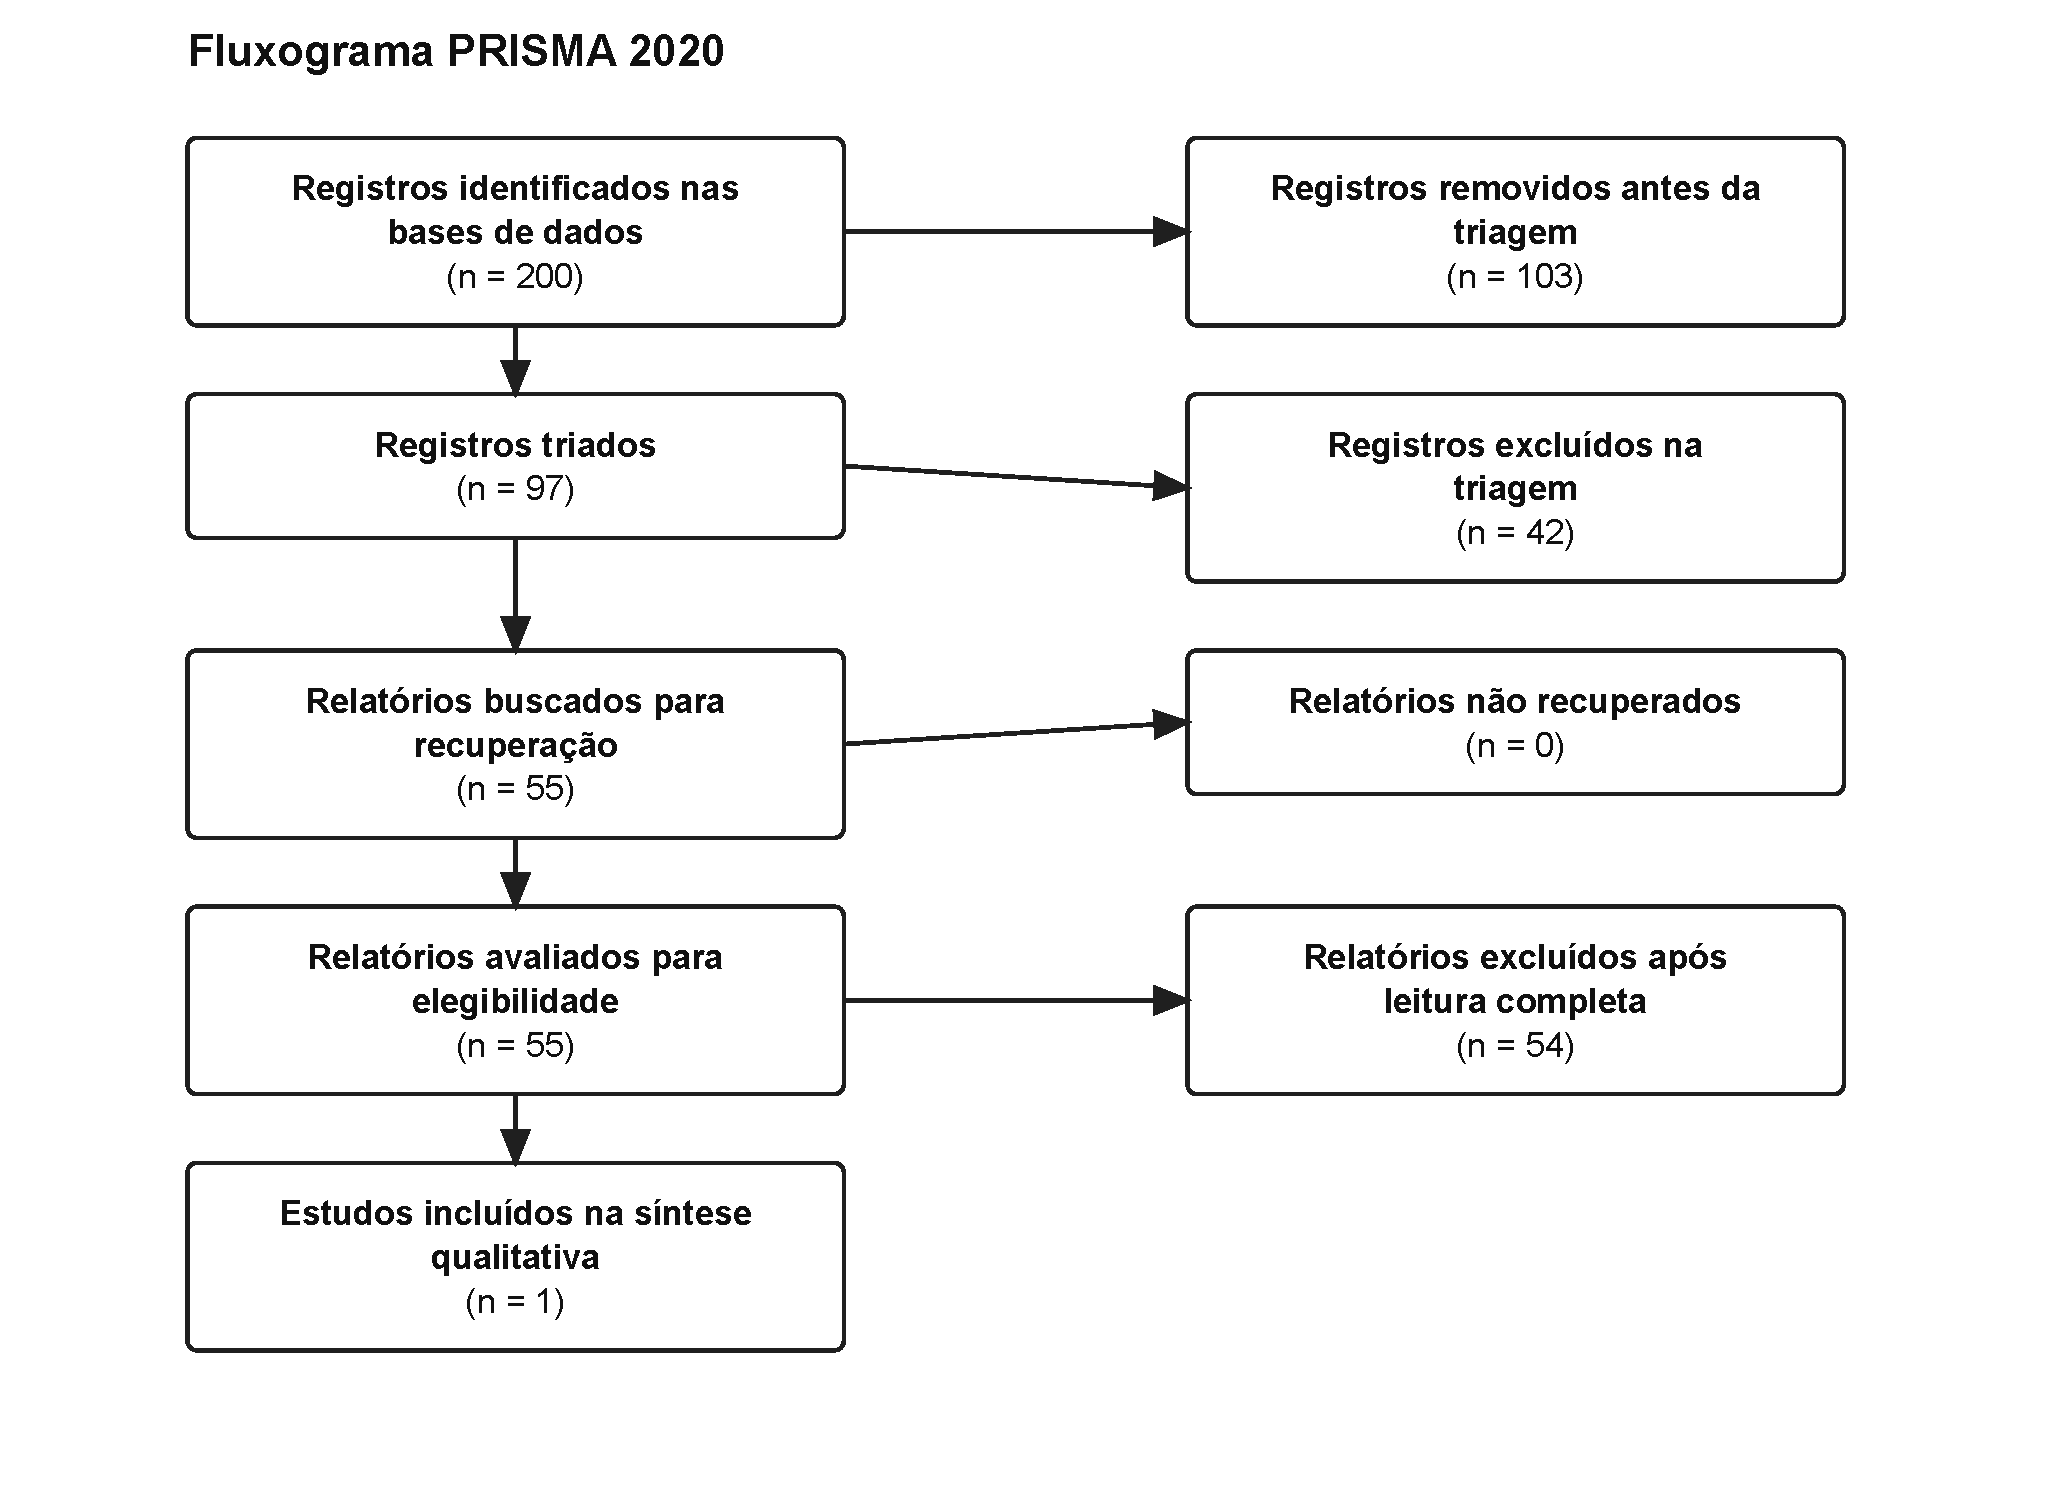
\includegraphics[width=0.78\textwidth]{atividade_uso_da_inteligencia_artificial_na_administracao_publica_federal_em_governanca_integridade_e_gestao_de_riscos_prisma_prisma.pdf}
\captionof{figure}{Fluxograma PRISMA 2020 da seleção do artigo de revisão sobre Uso da inteligência artificial na administração pública federal em governança, integridade e gestão de riscos.}
\label{fig:prisma2020_fluxo}
\end{center}

\section{Resumo do artigo selecionado}
\label{sec:orgc64a53f}

\subsection{Referência do estudo}
\label{sec:org050e9a9}

A referência do estudo selecionado corresponde a \autocite{freire2025automating}.

Freire, F. S., Costa, G. P. C. L., Martins, V. M., \& Saraiva, M. C. C. M. (2025). Automating public governance oversight: Evidence from the Federal District of Brazil. \textbf{Administratie si Management Public, 45}, 91–109. \url{https://doi.org/10.24818/amp/2025.45-05}

\subsection{Link para download do texto completo}
\label{sec:org02f4267}

\href{https://ramp.ase.ro/vol45/45-05.pdf}{Download do PDF}

\subsection{Problema e objetivo de pesquisa}
\label{sec:orgc035576}

O estudo investiga em que medida a automação baseada em inteligência artificial e web scraping pode apoiar a supervisão da governança pública e da transparência administrativa, tomando como objeto empírico a publicação de atas dos Comitês Internos de Governança (CIGs) por órgãos e entidades do Distrito Federal. O problema central decorre da percepção de lacunas na institucionalização da governança e da integridade, expressas na ausência de estruturas formais, na baixa padronização da divulgação de informações e na insuficiente digitalização de processos, o que compromete o monitoramento, a accountability e a maturidade institucional.

\subsection{Argumento central}
\label{sec:orga49beba}

O argumento central do artigo é que a automação de rotinas de coleta, verificação e classificação de dados públicos, quando combinada com inteligência artificial e técnicas de web scraping, pode fortalecer a governança, a transparência e a responsabilização no setor público. Os autores sustentam que o sistema LARA constitui um modelo replicável de accountability automatizada, capaz de identificar falhas de conformidade e apoiar o controle de práticas de governança, desde que acompanhado por padronização institucional, qualificação de servidores, mecanismos de auditoria e maior digitalização dos registros administrativos.

\subsection{Desenho de pesquisa}
\label{sec:org9430658}

Trata-se de um estudo empírico com abordagem de métodos mistos. O universo analisado compreende 47 organizações públicas do Distrito Federal, selecionadas a partir da Lei Orçamentária Anual de 2023, incluindo órgãos da administração direta, autarquias, fundações públicas, empresas públicas e sociedades de economia mista. O desenho metodológico combinou: (a) análise documental do arcabouço normativo e dos registros institucionais de governança; (b) extração automatizada de dados em sítios eletrônicos por meio do bot LARA, desenvolvido em Python; e (c) validação de conteúdo dos links e registros localizados. O LARA emprega requisições HTTP, parsing de HTML, filtragem e comparação de dados para identificar a existência de atos institucionais, composição dos CIGs e publicação de atas. A análise classificou as entidades em grupos de conformidade segundo a existência e a institucionalização das práticas de governança.

\subsection{Principais achados}
\label{sec:orgfb88c33}

Os principais achados indicam que há deficiências relevantes na governança e na transparência institucional. Entre as 47 entidades analisadas, 27,7\% não possuíam evidências de estrutura formal de governança, isto é, não apresentavam ato de instituição do CIG, designação de membros nem registros de transparência. Apenas 57,4\% alcançaram conformidade plena, com ato normativo, membros designados e atas publicadas para 2024 e 2025. Outros 6,4\% possuíam estrutura formal, mas sem publicação de atas, e 8,5\% publicavam atas apenas até anos anteriores a 2024, sugerindo institucionalização incompleta. O LARA apresentou desempenho satisfatório, com acurácia geral de 73,53\% na identificação de órgãos com ato de criação e membros definidos; no grupo de conformidade plena, a acurácia foi de 74,07\% para atos e composição e 77,78\% para atas. Os resultados mostram que a fragmentação institucional, a baixa padronização e a limitada digitalização dificultam a efetividade da governança e do monitoramento automatizado.

\subsection{Justificativa da seleção final}
\label{sec:org5dd8fa9}

O artigo justifica sua seleção final por atender integralmente aos critérios da atividade. Em primeiro lugar, é um estudo empírico, com aplicação concreta de uma ferramenta automatizada em organizações públicas brasileiras. Em segundo lugar, examina diretamente o uso da inteligência artificial e da automação no apoio à governança pública, à integridade e ao monitoramento de conformidade, elementos centrais do recorte temático proposto. Em terceiro lugar, apresenta resultados mensuráveis, com universo definido, procedimento metodológico explícito e achados quantitativos e qualitativos relevantes. Embora o caso empírico se concentre no Distrito Federal, o estudo dialoga com normativos e referenciais da administração pública brasileira, inclusive o Decreto nº 9.203/2017 e orientações do TCU, o que amplia sua pertinência para a administração pública federal. Por fim, o artigo possuía link verificável e funcional para download do texto completo em PDF, condição obrigatória para inclusão nesta etapa analítica.

\subsection{Contribuição do estudo para o tema}
\label{sec:org32dc655}

O estudo contribui para a literatura sobre governança digital ao oferecer evidência empírica do uso de automação e inteligência artificial como instrumentos de apoio ao monitoramento da governança pública. Sua principal contribuição está em propor e testar um modelo replicável de accountability automatizada para avaliação da transparência ativa e da conformidade institucional. Para o campo temático desta atividade, o artigo é particularmente relevante porque articula IA, governança, integridade e gestão de riscos de modo aplicado: a ferramenta automatizada permite detectar vulnerabilidades institucionais, apoiar controles preventivos, ampliar a visibilidade sobre práticas de governança e subsidiar decisões corretivas. Ainda que o foco imediato recaia sobre transparência e supervisão de comitês de governança, o estudo dialoga diretamente com a gestão de riscos ao evidenciar como a ausência de registros, padronização e rotinas digitais aumenta riscos de opacidade, descontinuidade e baixa capacidade de controle.

\section{Texto corrido para entrega}
\label{sec:org719bdc0}

Freire, Costa, Martins e Saraiva (2025) analisam como a automação pode fortalecer a transparência e a governança no setor público brasileiro a partir do desenvolvimento e da aplicação do sistema LARA no Distrito Federal. O problema investigado decorre da existência de lacunas institucionais na formalização e na operacionalização de mecanismos de governança, especialmente na publicação de atas dos Comitês Internos de Governança, elemento entendido pelos autores como evidência de institucionalização, transparência ativa e accountability. Nesse sentido, o estudo parte da premissa de que ferramentas baseadas em inteligência artificial e web scraping podem apoiar o monitoramento da conformidade institucional e ampliar a capacidade estatal de supervisão.

O argumento central do artigo sustenta que a automação do acompanhamento de registros públicos de governança pode modernizar a supervisão administrativa, aumentar a transparência e contribuir para a responsabilização institucional. Para os autores, o sistema LARA representa um modelo replicável de accountability automatizada, desde que sua adoção venha acompanhada de maior padronização dos dados, digitalização dos processos, treinamento de pessoal e mecanismos de auditoria que assegurem acurácia e explicabilidade.

Metodologicamente, trata-se de um estudo empírico com abordagem de métodos mistos. Os autores selecionaram 47 órgãos e entidades do Distrito Federal com base na Lei Orçamentária Anual de 2023, abrangendo administração direta, autarquias, fundações, empresas públicas e sociedades de economia mista. O desenho de pesquisa articulou análise documental, extração automatizada de dados em páginas eletrônicas institucionais e validação do conteúdo coletado. O sistema LARA, desenvolvido em Python, realiza buscas automatizadas, filtra links, compara os dados extraídos com registros estruturados e verifica a existência de atos de instituição dos comitês, composição de membros e publicação de atas.

Os resultados revelam fragilidades importantes na governança institucional. Entre as 47 entidades examinadas, 27,7\% não apresentaram qualquer evidência de estrutura formal de governança, isto é, não possuíam ato de criação do comitê, membros designados ou registros públicos associados. Apenas 57,4\% atingiram o nível de conformidade plena, com estrutura formalizada e atas atualizadas para 2024 e 2025. Além disso, 6,4\% apresentaram institucionalização parcial, com estrutura constituída, mas sem divulgação de atas, e 8,5\% publicavam atas apenas relativas a anos anteriores, o que indica descontinuidade ou insuficiência na transparência. O LARA obteve acurácia geral de 73,53\% na identificação de estruturas formais e, no grupo de maior conformidade, apresentou 74,07\% de acerto para atos e membros e 77,78\% para atas.

A principal contribuição do estudo está em demonstrar, de forma aplicada, que a inteligência artificial pode servir como instrumento de apoio à governança, à integridade e à gestão de riscos na administração pública. Embora o foco empírico esteja na transparência e no controle da publicação de atas, o artigo evidencia que a automação ajuda a identificar riscos institucionais associados à opacidade, à fragmentação organizacional, à baixa padronização e à limitada maturidade digital. Desse modo, a IA aparece não como substituta da decisão pública, mas como suporte ao monitoramento, à detecção de falhas de conformidade e ao fortalecimento de mecanismos de controle e accountability.

O artigo foi adequadamente selecionado para compor a atividade acadêmica porque atende ao objetivo de identificar e analisar um estudo empírico sobre o uso da inteligência artificial na administração pública. Além de tratar diretamente de governança, integridade e monitoramento de conformidade, apresenta base empírica clara, resultados verificáveis e potencial de replicação em outros contextos governamentais. Ainda que o estudo se concentre no Distrito Federal, sua discussão normativa e institucional dialoga com referenciais da administração pública federal, o que reforça sua pertinência analítica. Soma-se a isso o fato de o texto completo estar disponível por link verificável para download, satisfazendo o requisito metodológico de elegibilidade da atividade.

\printbibliography
\end{document}